\documentclass{scrartcl}
\usepackage[utf8]{inputenc}
\usepackage{graphicx}
\title{Project: Power Cloud}
\subtitle{Client: Hanrich Potgieter \\ Team: Quadcore Productions\\}
\author{Themba Mbhele 14007950\\ Moses Mayimela 14019702 \\ Hlengekile Jita 14077893 \\ Mpho Baloyi 14133670 \\Department of Computer Science, University of Pretoria}
\date{01 May 2016}


\begin{document}

\maketitle
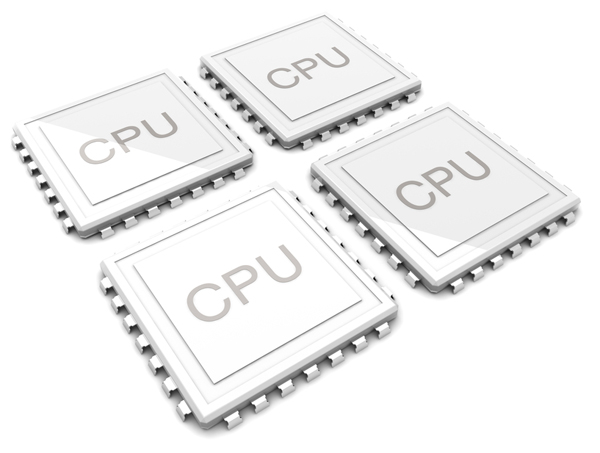
\includegraphics[width=\textwidth]{2012-quad-core-phones}
\section{The Team}
\subsection{Moses Mayimela}
\subsection{Hlengekile Jita}
\subsection{Mpho Baloyi}
\subsubsection{Interests}
\begin{itemize}
\item Keeping abreast with new technologies
\item Learning and using new technologies to solve problems
\item Reading up and doing research on new and old concepts in computer science
\item Solving riddles and puzzles
\item Helping people through ICT
\end{itemize}
\subsubsection{Technical Skills}
\begin{itemize}
\item Solid programming skills in java,c++ and python
\item Fair amount of knowlegde in assembly programming 
\item Web development with HTML,JAVASCRIPT,JQUERY,CSS,PHP,AJAX,ANGULARJS
\item Interaction Design 
\item Database design with MySQL
\item Understanding of process development
\item Unit testing,mocking and dependency Injection
\end{itemize}
\subsubsection{Non-technical Skills}
\begin{itemize}
\item Exellent Communication skills
\item Patient 
\item Creative approach to problem solving
\item Pay attention to detail 
\item Excellent planning skills
\item Ability to grasp concepts quickly
\item Willness to learn new things
\item Ability to interpret and follow technical plans
\item Ability to collaborate and work efficiently with other people
\item Ability to work under pressure
\end{itemize}
\subsubsection{What makes you want to do the project}
\begin{flushleft}
My interest and deep passion for Internet of Things,helping people and more importantly providing people with means to take
care of the enviroment through careful power consumption are the main reasons why I want to do this project. I also want to do
this project because it is an opportunity to learn and see how software and hardware work togther which has always been one of my many interests.The project presents an opportunity to learn new things,acquire new skills and refine my skills and I believe this is the headstart i need for my career in Computer Science. 
\end{flushleft}
\subsection{Themba Mbhele}

\section{Project Execution}
\subsection{Development Methodology}
\subsection{Communication With Client}
To keep the clients informed we are going to use the following means of communication
\subsubsection{email}
\begin{itemize}
\item To inform the client of our progress
\item To address any issues or concerns that they client may have
\item To acquire information from the client
\item To require any resources that the client has to offer for their project,..
\end{itemize}

\subsubsection{Phone calls}
 This will only be used to address very urgent matters if they arise during the course of the project development 
 however this will only be done with permission from the client and during business hours.
 
\subsubsection{Regular Meetings}	 
These will take place depending on the clients availiability and willness.
We may discuss the progress of the project,to address any concerns,etc.

\subsubsection{GIT}

Access to our git repository will be provided to the client,so the client can be able to monitor
our progress and have access to the project material.

We are also open to any means of communicatiuon that the client may prefer or suggest.

\subsection{Technical Challenges}
\subsubsection{Collecting the readings}
The sensors or hardware that will be used to collect the physical readings have not been outlined and thus the challenge is how these values will be captured from the operating machinery.\\ \\
The solution:\\ 
Since the boards (photon and electron) have GPIOs, these can be used to interface with the various sensors that will capture the readings such as voltage and current. To measure current, a Current transformer, for example can be used to capture the operating current of a machine.\\
\\
To measure voltage, a step down transformer can be used to step down the voltage of the line connected in parallel to the operating machine. once the voltage has been stepped down to a level that the boards can tolerate i.e the max voltage would be 3.3V logic since the boards can operate at 3.3V VCC, then the signal can be fed to the analog pins of either the photon or the electron board.
\\ \\
These values, voltage and current are essential for the computation of other values such as power, e.g P=VI. 

\subsubsection{Connecting the photon to a local router}
The electron has a direct connection to the internet through the SARA-U260 module. The photon board, however needs a mobile device to get internet connection and thus thus the challenge will be to eliminate the need for a cellphone for the internet connection.\\ \\
The solution:\\
The approach to follow is to use a device that can connect more than one device to the internet e.g a wifi router. The router can provide all the photon boards with a connection to the internet. 
\subsection{Technologies}
This section will list the technologies that will be used to implement the system.\\
To implement the back-end of the system, the following technologies will be used:
\begin{itemize}
    \item NodeJS will be used to implement the server.
    \item MongoDB will be used to store the data that will be collected.
    \item C++ will be used to program the hardware
\end{itemize}
To implement the front-end of the system, the following technologies will be used:
\begin{itemize}
    \item AngularJS will be used for the web front-end.
\end{itemize}

\end{document}
